The goal is to combine both data sets, transform them when necessary to reduce size, features and use them with ML training algorithms that enable an accurate cryptocurrency market price prediction.

\subsection{Cryptocurrency data set processing}

Because this data set was machine-generated little had to be done to process it. It was important, however, to examine the contained information and extract just the necessary one in real time. Because of data size, and the technical resources limitations it was not possible to extract and store the required information, but rather open the file, select the main features and use them in real time for machine learning algorithm to train and generate a model, and the close it. Uncompressed data reached 70 GB of space, whereas compressed data set just 9 GB.

\subsubsection{Data set description and feature selection}
Each parquet file in the data set contains the corresponding information as shown in Figure 5. 


\begin{figure}[H]
   \centering
   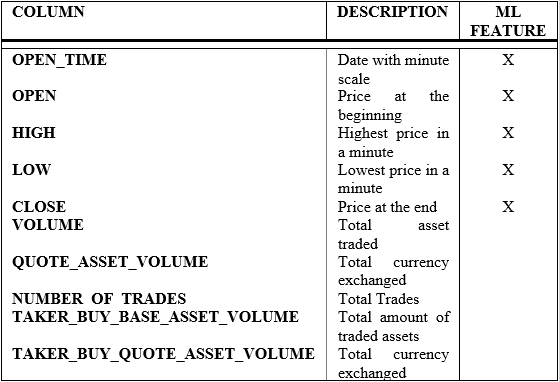
\includegraphics[width=\linewidth]{fig/Cryptocurrency features.png}
    \caption{Cryptocurrency features}
    \label{fig:CryptocurrencyFeatures}
\end{figure}

\begin{figure}[H]
   \centering
   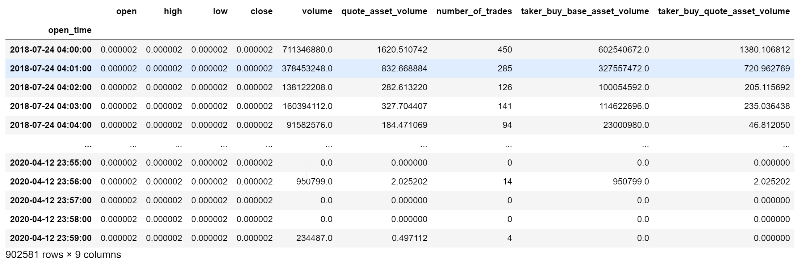
\includegraphics[width=\linewidth]{fig/ExampleParquetFile HOT-ETH.png}
    \caption{Example of parquet file HOT-ETH.parquet}
    \label{fig:CryptocurrencyDataSetParquetFile}
\end{figure}

From \ref{fig:CryptocurrencyFeatures} features marked with ‘X’ where selected to be processed and to train the Machine Learning model.

\subsection{Cryptocurrency news data processing}
This data set was non-existent, it had to be generated by creating a python script to bring the information from the web portal “coinmarketcap.com”. The script uses web scraping methodology and extracts the news set according to the given parameters.  
A total of 24519 news articles had to be gathered and processed to generate the data set in two steps.
The first step consists on getting the header information from the web portal, whereas the second brings the content of a specific  news article.
 The script was generated and run in a Hadoop cluster to better control and preserve information in case of data loss. 
A part of the algorithm is shown, full code description and implementation can be seen in \cite{christopher_olah_understanding_2015}.

\begin{figure}[H]
   \centering
   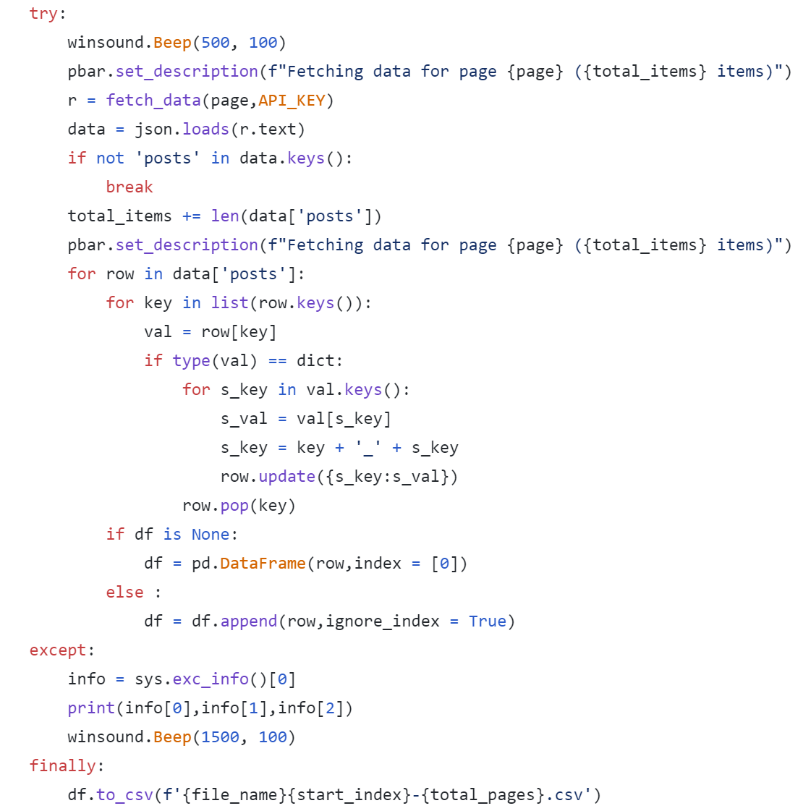
\includegraphics[width=\linewidth]{fig/CodeSnippetNewsHeading.png}
    \caption{Code implementation for news heading extraction. Data is extracted into a dictionary and later saved on a pandas DataFrame}
    \label{fig:CodeSnippetNewsHeading}
\end{figure}

\begin{figure}[H]
   \centering
   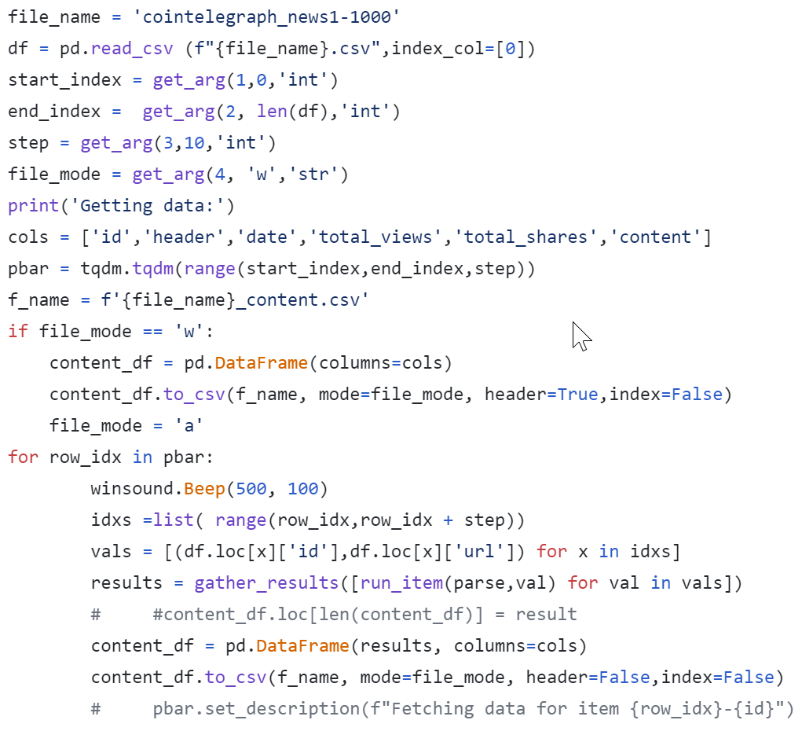
\includegraphics[width=\linewidth]{fig/CodeSnippetNewsContent.png}
    \caption{Code implementation for news article extraction, data is directly saved in a pandas DataFrame and updated in a csv file. http request interactions are intensive and took close to 3 days of continuous execution to retrieve the full data set}
    \label{fig:CodeSnippetNewsContent}
\end{figure}

Once created the data set, it was properly cleaned and processed to be used for natural language processing just one file (cointelegraph\textunderscore news\textunderscore content.csv) was used to train the model for being the one with the article content.

\begin{figure}[H]
   \centering
   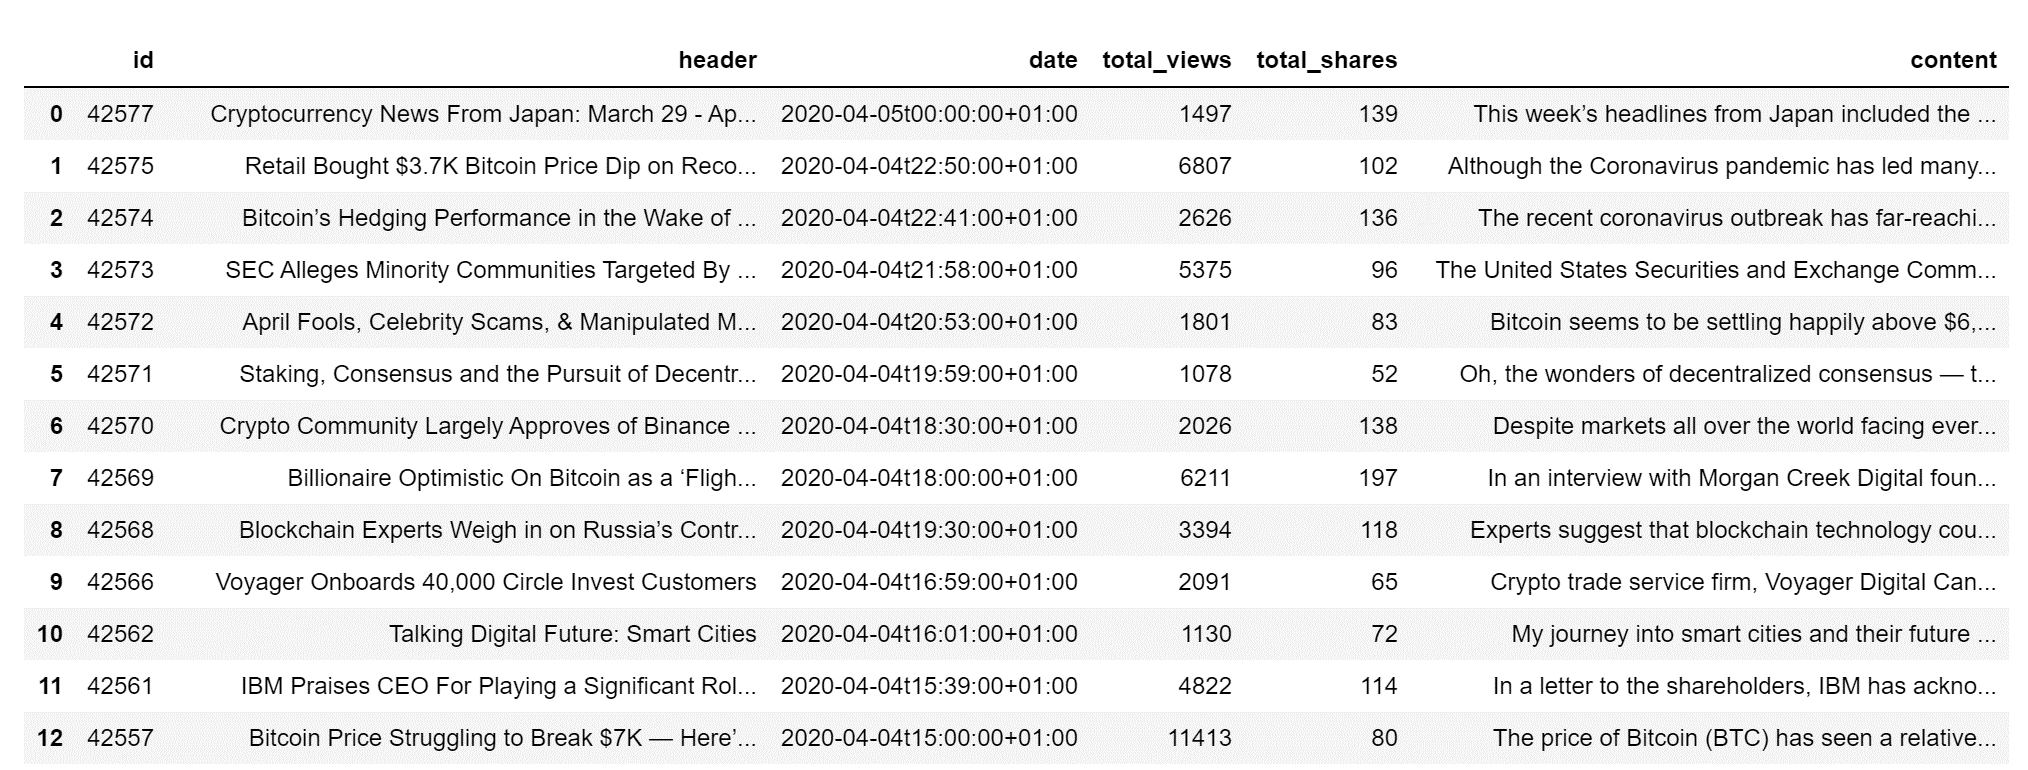
\includegraphics[width=\linewidth]{fig/NewsContentExample.png}
    \caption{Cryptocurrency news content example}
    \label{fig:NewsContentExample}
\end{figure}
